\section{Assignment 16.9}
\textbf{Assignment Description}
\begin{figure}[H]
	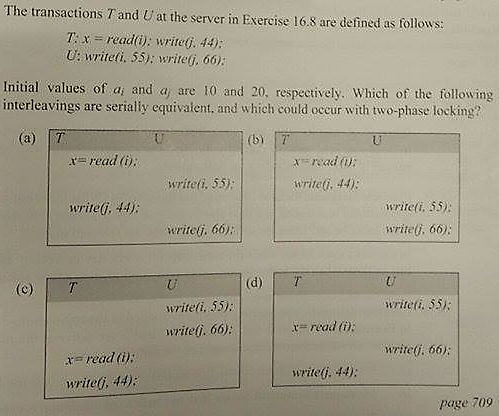
\includegraphics[width = \linewidth]{assignment169}
\end{figure}

a) and b) are serially equivalent, because the write operations on \textit{i} and on \textit{j} are equivalent to writing \textit{j} and \textit{i} since the operations happen on different objects and will not interfere. 
c) and d) are serially equivalent, because reading \textit{i} and writing \textit{j} in d) is equivalent to writing to \textit{j} and reading \textit{i} as in c), since the action happens on different objects, which do not interfere with each other.\\\\
The 2-phase-locking protocol states that a transaction must handle its locks in two distinct, consecutive phases during the transaction's execution:
\begin{enumerate}
	\item \textbf{Expanding phase}' (aka Growing phase): locks are acquired and no locks are released (the number of locks can only increase).
	\item \textbf{Shrinking phase}: locks are released and no locks are acquired.
\end{enumerate}
therefore only b) and c) could occur with two-phase locking. As an example of why a) or b) could not occur one could look at a, where \textit{T} needs to acquire a lock to read \textit{i}, then it needs to release the lock for \textit{U} to use it, but then another lock is acquired for \textit{T} to make a write to \textit{j}. This is not allowed according to the 2pl protocol.